\documentclass[12p,a4paper]{report}
\usepackage[utf8]{inputenc}
\usepackage[T1]{fontenc,url}
\usepackage{parskip}
\usepackage{lmodern}
\usepackage{microtype}
\usepackage{verbatim}
\usepackage{amsmath, amssymb}
\usepackage{tikz}
\usepackage{physics}
\usepackage{mathtools}
\usepackage{algorithm}
\usepackage{algpseudocode}
\usepackage{listings}
\usepackage{enumerate}
\usepackage{graphicx}
\usepackage{float}
\usepackage{epigraph}
\usepackage{hyperref}
\usepackage{minted}
\usepackage{siunitx}
\usepackage[margin=3.5cm, include headfoot]{geometry}

%\usemintedstyle{vim}
\newminted{python}{frame=lines,framerule=2pt}  %Enables frame option for minted.

\begin{document}

\renewcommand{\exp}{\mathrm{e}^}

\title{FYS2130 - Prosjektoppgave}
\author{
		Kandidatnummer 15004
		}
\maketitle
\pagebreak

\setcounter{page}{1}
\section*{Oppgave 1}
\subsubsection*{Diskretisering og notasjon}
Vi diskretiserer systemet som $N$ massepunkter $m_i$ av varierende masse, som er bundet sammen av $N-1$ strenger av varierende styrke $k_i$. Videre diskretiserer vi massepunktenets utslag fra likevektslinjen $y=0$ som $y_i$.

For å representere et tidssteg fremover og bakover i tid fra tidspunktet $t$, bruker vi den følgende diskretisering: $y(x_i,t+\Delta t) = y_i^+$, $\ y(x_i, t) = y_i^0$ og $\ y(x_i, t-\Delta t) = y_i^-$, 

Vi bruker denne diskretiseringen til å sette opp Newtons andre lov for hvert massepunkt:
\begin{align}\label{eqn:newton}
	F_i = m_i\ddot{y_i}
\end{align}

\subsubsection*{Utlede bevegelsesligningen}
I appendiks A har jeg utledet ligning \ref{eqn:yder} (ligning (O.2) fra oppgaven), fordi jeg synes utledningen er vakker, og det gir oss dessuten informasjon om feilledded som kommer fra tilnærmingen. Resultatet er gitt som
\begin{align}\label{eqn:yder}
\ddot{y}_i^0 \approx \frac{y_i^+ - 2y_i^0 + y_i^-}{\Delta t^2}
\end{align}
der vi har har en presisjonsfeil som går som $\Delta t^4$. Dette kan vi bruke til å tilnærme høyresiden i ligning \ref{eqn:newton}

Den totale kraften $F_i$ som virker på et punkt $i$ er utledet i oppgaven (ligning (O.1)) som
\begin{align}\label{eqn:F}
F_i = -(k_{i-1} + k_i)y_i + k_{i-1}y_{i-1} + k_iy_{i+1}
\end{align}

Hvis vi setter ligning \ref{eqn:F} og \ref{eqn:yder} inn i ligning \ref{eqn:newton}, kan vi løse for $y_i^+$:

\begin{align*}
m_i\qty(\frac{y_i^+ - 2y_i + y_i^-}{\Delta t^2}) &= -(k_{i-1} + k_i)y_i + k_{i-1}y_{i-1} + k_iy_{i+1}
\\
y_i^+ - 2y_i + y_i^- &= \alpha_i\qty[-(k_{i-1} + k_i)y_i + k_{i-1}y_{i-1} + k_iy_{i+1}]
\\
y_i^+ &= \alpha_i\qty[-(k_{i-1} + k_i)y_i + k_{i-1}y_{i-1} + k_iy_{i+1}] + 2y_i - y_i^-
\end{align*}
Der vi har introdusert variablen $\alpha_i = \Delta t^2/m_i$.

For de tilfellene der vi har konstant fjærstivhet over hele systemet, vil $k_i = k$ for alle $i$, og vi kan videre forenkle uttrykket til
\begin{align*}
y_i^+ &= \alpha_i\qty[-(k + k)y_i + ky_{i-1} + ky_{i+1}] + 2y_i - y_i^- \\
y_i^+ &= \beta_i\qty[-2y_i + y_{i-1} + y_{i+1}] + 2y_i - y_i^-
\end{align*}
Der vi har introdusert variabelen $\beta_i = k \Delta t^2/m_i$

\subsubsection*{Randbetingelser}
Denne ligningen vil gjelde for $i \in [1,\ N-2]$, altså for alle punkter med unntak av randpunktene, $y_0$ og $y_{N-1}$. Disse to punktene vil bare oppleve en kraft fra én fjær, som betyr at kraftformelen \ref{eqn:F} vi har benyttet ikke gjelder. Vi kan skrive om denne til å bare inkludere krefter fra én side, og gjøre utledningen av $y_i^+$ på nytt. Dette resulterer i følgende ligninger for de to endepunktene:
\begin{align*}
y_0^+ = \alpha_i\qty[-k_{i}y_i + k_{i}y_{i+1}] + 2y_i - y_i^-\\
y_N^+ = \alpha_i\qty[-k_{i-1}y_i + k_{i-1}y_{i-1}] + 2y_i - y_i^-
\end{align*}

En lukket randbetingelse oppstår når vi får en enorm (i teorien uendelig) impedansøkning på randpunktene. Dette vil bety at randpunktene forblir ved ved 0: $y_0 = y_{N-1} = 0$. I praksis skjer dette gjerne når endene er festet i noe solid, som en vegg, som selvsagt har en enorm masse. Vi ser at dersom $m<<0$ vil $\alpha << 1$, som fører til at $y_i^+ \approx y_i^0$, og endepunktene står stille. Fordi punktene i teorien skal stå stille uansett, har jeg valgt å bare la dem forbli på $y = 0$ i våre simuleringer. Dette gir identiske resultater, er enklere å implementere, mindre ressurskrevende, og forhindrer kombinasjoner av enormt store og små floats, som er en dårlig programmeringspraksis.

For en åpen randbetingelse vil randpunktene bevege seg som normalt, etter formlene vi utledet ovenfor. Dette betyr altså at vi må oppdatere randpunktenes posisjon på samme måte alle andre punkter, men med den spesielle formelen.



\section*{Oppgave 2}
Vi tar vår diskretiserte newtons andre lov, ligning \ref{eqn:newton}, og setter inn vårt uttrykk for kraften på et massepunkt fra ligning \ref{eqn:F}:
\begin{align*}
F_i &= m_i \ddot{y} \\
-(k_{i-1} + k_i)y_i + k_{i-1}y_{i-1} + k_iy_{i+1} &= m_i \frac{\partial^2 y}{\partial t^2}
\end{align*}

Ved konstant massetetthet får vi at $m_i = m = \mu \Delta x$, og ved konstant fjærstivhet får vi at $k_i = k = \kappa/\Delta x$. Vi setter inn for disse, og får
\begin{align*}
-2\frac{\kappa}{\Delta x} y_i + \frac{\kappa}{\Delta x}y_{i-1} + \frac{\kappa}{\Delta x}y_{i+1} &= \mu \Delta x \frac{\partial^2 y}{\partial t^2} \\
\\
\frac{y_{i+1} - 2y_i + y_{i-1}}{\Delta x^2}\frac{\kappa}{\mu} &= \frac{\partial^2 y}{\partial t^2}
\end{align*} 

Ligning \ref{eqn:yder} gir oss en tilnærming til den dobbelt tidsderiverte av $y$. Vi ser at venstresiden i ligningen over er en tilsvarende tilnærming til den dobbelt x-deriverte av $y$, altså på formen
\begin{align*}
\frac{y_{i+1} - 2y_i + y_{i-1}}{\Delta x^2} \approx \frac{\partial^2 y}{\partial x^2}
\end{align*}
der vi viste at feilen vil gå som $\Delta x^4$. Fordi vi har en konstant massefordeling vil vi i teorien ha uendelig mange massepunkter, og uendelig liten $\Delta x$, som betyr at feilen går raskt mot 0.

Setter vi inn for tilnærmingen, blir ligningen på formen
\begin{align*}
\frac{\partial^2 y}{\partial x^2}\frac{\kappa}{\mu} = \frac{\partial^2 y}{\partial t^2}
\end{align*}

Vi ser altså at vi har utledet bølgeligningen for systemet vårt, der hastigheten til bølgen er git som
\begin{align}\label{eqn:vB}
v_B = \sqrt{\frac{\kappa}{\mu}}
\end{align}


\section*{Oppgave 3}
Vi har bølgens utbredelseshastighet definert i ligning \ref{eqn:vB}. Hvis vi setter inn for $\kappa = k\Delta x$ og $\mu = m/\Delta x$ får vi
\begin{align*}
v_B = \sqrt{\frac{k\Delta x}{m/\Delta x}} = \sqrt{\frac{k}{m}}\Delta x
\end{align*}

Som oppgaven sier, må vi oppløse beregningene våre med en hastighet $\Delta x/\Delta t$ som er større enn bølgens hastighet, for å unngå et ustabilt system. Vi får altså at
\begin{align*}
\frac{\Delta x}{\Delta t} \geq v_B \\
\frac{\Delta x}{\Delta t} \geq \sqrt{\frac{k}{m}}\Delta x \\
\end{align*}

Vi kan løse for dette for $\Delta t$, for å se hva slags kriterier vi har for tidsstegene våre:
\begin{align}\label{eqn:dt}
\Delta t \leq \sqrt{\frac{m}{k}}
\end{align}

Vi observerer altså at $\Delta x$ er irrelevant for vår numeriske presisjon. Dette er ikke så unaturlig, ettersom vi har modellert systemet vårt til å bare ha krefter i y-retning, og hvor langt vi definerer det å være mellom hvert massepunkt vil ikke påvirke dette. Den vertikale bevegelsen til hvert massepunkt er altså helt uavhengig av x, og det er den vertikale posisjonsendringen som skaper bølgen.

Vi kunne faktisk definert alle hastigheter til å være i \textit{punkter} per sekund, istedenfor meter per sekund. Da hadde vi sett at all avhengighet av $x$ ville forsvunnet fra alle ligninger, uten at det ville by på noen problemer.

En annen måte å tenke på det på er at enhver økning i $\Delta x$ vil øke vår oppløsningshastighet og bølgens utbredelseshastighet akkurat like mye.



\section*{Oppgave 4}
\subsubsection*{Initialbetingelser og parametre}
For å kunne løse utbredelsen av en bølge over tid numerisk, er vi avhengig av informasjon om både bølgens inititalposisjon, og hvilken retning den utbrer seg i. Initialposisjonen til bølgen er gitt i formelen
\begin{align}
\label{eqn:sinus}
y_i^0 = \sin\qty(7\pi\frac{i}{N-1})
\end{align}
Informasjonen om bølgens hastighet er lagret i forholdet mellom $y_i^0$ og $y_i^-$. Hvis vi for eksempel velger $y_i^-$ som en sinusbølge forskjøvet til høyre eller venstre for $y_i^0$, vil dette indikere at bølgen er en planbølge som beveger seg bortover langs x-aksen. Akkurat denne bølgen (en sinusbølge av 3.5 perioder med reflekterende randbetingelser) vil det kanskje være mer naturlig å anse som en stående bølge, ettersom en planbølge ikke vil kunne oprettholde seg selv med reflekterende rander. Men jeg ønsker å påpeke at dette ikke er et entydig objektivt svar, og det hadde fint vært mulig å implementere andre bølgetyper, avhengig av de valgte initialbetingelsene. For en stående bølge vil altså bølgen ikke beveger seg langs x-aksen, som tilsvarer at $y_i^-$ ikke er forskjøvet i forhold til $y_i^0$ i x-planet. Den enkleste måten å implementere dette på vil rett og slett være å sette $y_i^- = y_i^0$, som betyr at vi starter simuleringen når den stående bølgen er på sitt maksimale utslag. Det ville også vært mulig å sette $y_i^-$ som en tilsvarende sinusbølge, bare litt lavere. Dette er riktignok mer avansert å implementere, og skal gi identisk resultat (utenom en forskyvning i tidsutviklingen av bølgen).

Vi har også parametrene vi trenger for å sette en betingelse på $\Delta t$. Denne vil altså være
\begin{align*}
\Delta t \leq \sqrt{\frac{m}{k}} = \sqrt{\frac{\SI{0.02}{kg}}{\SI{10}{kg/s^2}}} = \SI{0.0447}{s}
\end{align*}
Vi ønsker altså en verdi under $\SI{0.0447}{s}$, men heller ikke en for lav verdi, ettersom antallet tidssteg er bestemt, og vi ikke ønsker å simulere et ekstremt kort tidsintervall. Vi kan velge oss $\Delta t = \SI{0.01}{s}$ som et kompromiss.


\subsubsection*{Numerisk implementasjon og resultater}
Programmet bruker $y_i^- = y_i^0$ som initialbetingelser, og simulerer bevegelsen over de 1200 tidspunktene med tidssteg $\Delta t = \SI{0.01}{s}$. Fordi vi har konstant fjærstyrke og masse, initialiserer vi $\beta_i = k \Delta t^2/m_i$ utenfor tids-loopen, som vi beskrev i Oppgave 1. Koden lagrer \textit{ikke} alle tidsstegene i en fler-dimensjonal array, men beholder bare de relative tidspunktene $y^-$, $y^0$ og $y^+$, som oppdateres hver iterasjon. Dette sparer minne, men betyr riktignok at alle beregninger må gjøres i tids-loopen. Programmet er vektorisert, for å spare tid, men en ikke-vektorisert loop er også vedlagt (som er litt lettere å tolke).

Figur \ref{fig:sinus_wave} viser $y_i^0$ plottet over de første 1.3 sekundene, som tilsvarer en halv periode av bølgens oscillasjon. Tidspunktene $t=\SI{0}{s}$ og $t=\SI{1.3}{s}$ er markert med heltrukne linjer, mens jevnt fordelte tidspunkter imellom er plottet med stiplede linjer.

Figuren er ment å gi et best mulig inntrykk av hvordan bølgen utvikler seg over tid. Bølgen vil fortsette å oscillere mellom disse to ytterpunktene, så å plotte videre tidssteg vil bare gi et kaos av overlappende grafer.

\begin{figure}[H]
\centering
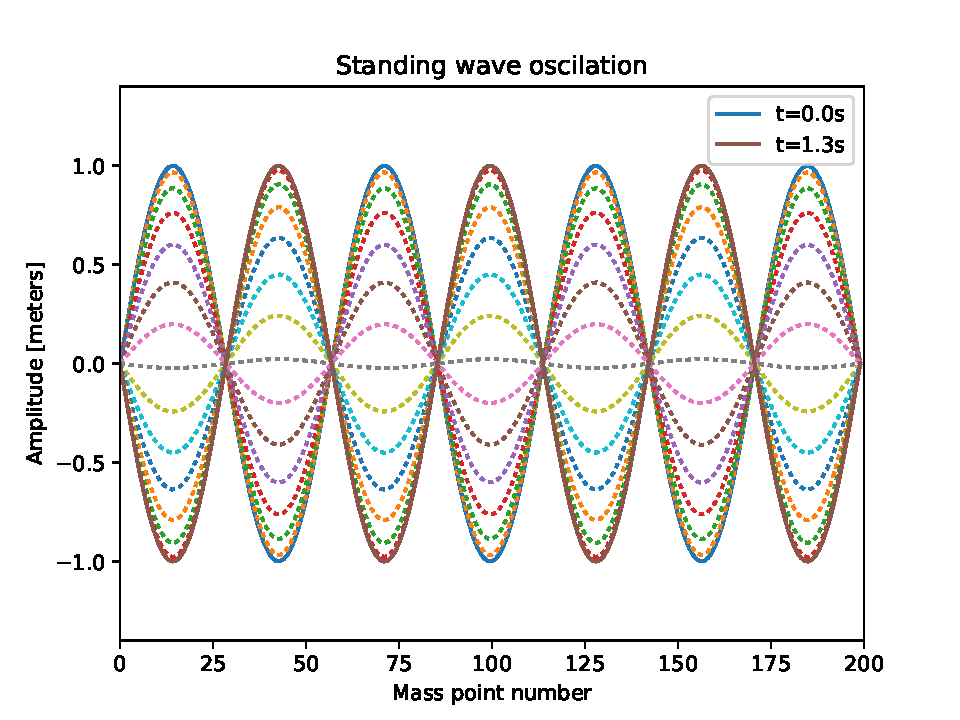
\includegraphics[width = \textwidth]{../fig/sinus_wave.pdf}
\caption{Stående sinusbølge over tid. De maksimale utslagene er markert i heltrukkede linjer.}
\label{fig:sinus_wave}
\end{figure}



\section*{Oppgave 5}
\subsubsection*{Analytisk løsning av frekvensen til det midterste massepunktet}
Vi skal nå plukke ut det midterste massepunktet, altså punkt $y_{99}$, og studere hvordan det utvikler seg over tid. Hvis vi tar en titt på sinusbølgen vår i figur \ref{fig:sinus_wave}, ser vi at det midterste punktet oscillerer med maksimal amplitude, fra -1 til 1. Det finnes andre punkter på sinuskurven som ikke beveger seg i det hele tatt, så det er greit å vite hva vi forventer. Vi kan starte med å regne ut hvilken frekvens vi forventer dette massepunktet å oscillere med, og deretter sjekke om dette stemmer med numeriske tester.

Hastigheten til en bølge kan defineres som produktet av bølgelengden og frekvensen:
\begin{align*}
v_B = \lambda f
\end{align*}
Setter vi inn vår løsning av $v_B$, og løser for frekvens, får vi
\begin{align*}
\sqrt{\frac{k}{m}} = \lambda f\\
f = \frac{1}{\lambda} \sqrt{\frac{k}{m}}
\end{align*}
$m$ og $k$ er kjente verdier, men hva er bølgelengden, $\lambda$? Hvis vi setter inn vår valgte $N = 200$ i ligningen for sinusbølgen \ref{eqn:sinus}, får vi
\begin{align*}
y_i^0 = \sin\qty(7\pi\frac{i}{199}) = \sin\qty(\frac{3.5}{199}2\pi i )
\end{align*}
Vi ser altså at frekvensen til sinusbølgen vår (i rom, ikke i tid!) er $\xi = 3.5/199$, som betyr at bølgelengden er $\lambda = 1/\xi = 199/3.5$.

På dette tidspunkt kan det være naturlig å fundere over hva slags enheter vi bruker her. Vanligvis ville den romlige frekvensen $\xi$ hatt enhet meter$^{-1}$, og bølgelengden hatt enhet meter. Men hvis vi ser på lengdevariabelen vi satte inn i sinusfunksjonen, $N=200$, så ser vi at den er enhetsløs. Den representerer bare et antall punkter, som er av vilkårlig lengde. Vi har altså skalert bort lengde i x-aksen, som er like greit, siden den ikke har en effekt på bevegelsen. Bølgelengden $\lambda$ er altså i enheten 'punkter', og den romlige frekvensen $\xi$ er i punkter$^{-1}$.

Vi setter inn for $\lambda = 199/3.5$, $m = \SI{0.02}{kg}$ og $k = \SI{10}{kg/s^2}$ og får
\begin{align}\label{eqn:ana_freq}
f = \frac{3.5}{199}\sqrt{\frac{\SI{10}{kg/s^2}}{\SI{0.02}{kg}}} \approx \SI{0.3933}{Hz}
\end{align}

Dette vil si at en periode er på $T = 1/f = \SI{2.5427}{s}$. Antallet tidssteg vi trenger for 10 perioder vil da bli
\begin{align*}
n\cdot \Delta t &= 10T\\
n = \frac{10T}{\Delta t} &= \frac{10\cdot \SI{2.5427}{s}}{\SI{0.01}{s}} = 2542.7 \approx 2542
\end{align*}
for vår valgte $\Delta t = \SI{0.01}{s}$.

\subsubsection*{Numerisk løsning av frekvensen til det midterste massepunktet}
Vi skal nå studere svingningen til det $y_{99}(t)$ numerisk. For å gjøre dette lager vi en ny array som lagrer utslaget til $y_{99}$ for hvert tidssteg vi gjør i loopen. Plotter vi dette mot tid får vi figur \ref{fig:100_point}, som viser utslaget til $y_{99}(t)$ over 2542 tidssteg med $\Delta t = 0.01$. Som vi ser svinger punktet også som en sinusbølge over tid! Vi ser også at punktet oscillerer 10 perioder over tidsintervallet vi har valgt, som var det vi ønsket.
\begin{figure}[H]
\centering
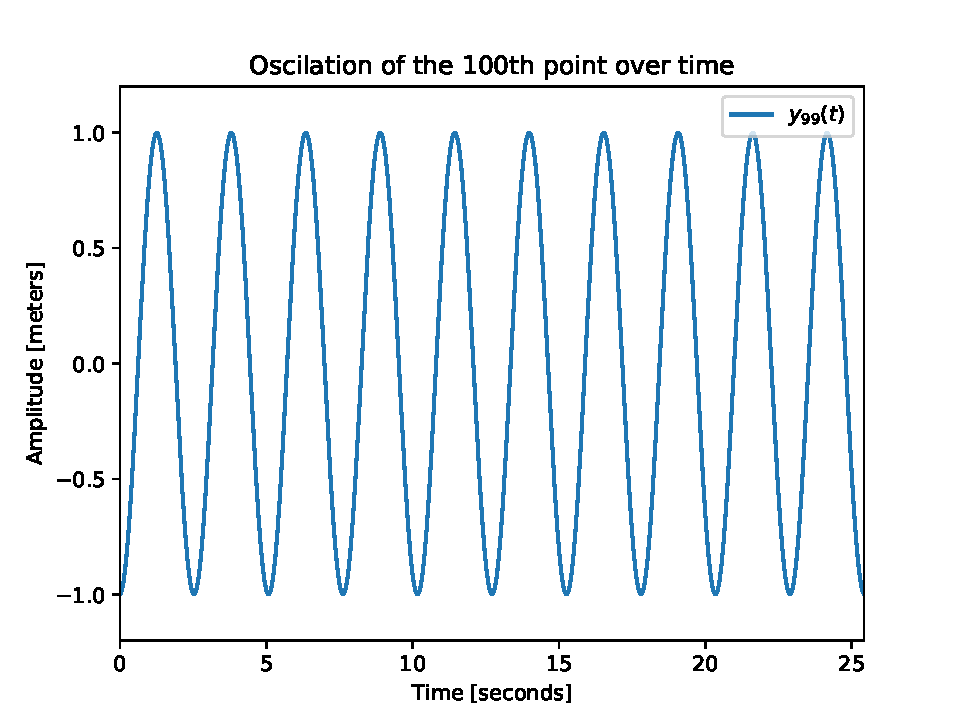
\includegraphics[width=\textwidth]{../fig/100_point_oscilation.pdf}
\caption{Utslaget til det midterste massepunktet $y_{99}$, plottet over tid}
\label{fig:100_point}
\end{figure}

For å finne frekvensen til denne svingningen kan vi studere avstanden mellom toppunktene. Numpy kan finne indeksene til lokale maksima i arrayet vi laget, og vi kan kombinere dette med vår valgte $\Delta t$ for å finne perioden, som forteller oss frekvensen:
\begin{align*}
f = \frac{1}{T} = \frac{1}{\Delta t \Delta A_{max}}
\end{align*}
der $\Delta A_{max}$ er avstanden mellom toppunktene til grafen.

Implementerer vi dette i programmet vårt får vi følgende frekvens mellom hvert toppunkt:
\begin{lstlisting}[frame = single]
Frequency between each maxima:  [ 0.39370079  0.39370079  0.39215686  0.39370079  0.39215686  0.39370079
  0.39370079  0.39215686  0.39370079]	
\end{lstlisting}
Som vi ser er det liten variasjon i frekvensene mellom hvert toppunkt, som er et godt tegn. De små variasjonene skyldes bare det begrensede antallet massepunkter. Tar vi gjennomsnittet av disse frekvensene får vi
\begin{lstlisting}[frame = single]
Average frequency of whole wave: 0.3932 Hz
\end{lstlisting}
Vår analytiske løsning av frekvensen er altså $f_{num} = \SI{0.3932}{Hz}$, mens vår analytiske løsning fra ligning \ref{eqn:ana_freq} var $f_{ana} = \SI{0.3933}{Hz}$. Dette er altså en relativ feil på
\begin{align*}
Error = \frac{|f_{ana} - f_{num}|}{f_{ana}} = \frac{0.0001}{0.3933} = 0.000254
\end{align*}
Som er en feil på under $0.2\%$, som er meget bra.



\subsubsection*{Fourier transformasjon av det midterste massepunktet}
Numpy kan fouriertransformere $y_{99}(t)$ for oss, ved hjelp av sin Fast Fourier funksjon \texttt{numpy.fft.fft()}. Plotter vi resultatet mot frekvensspekteret, får vi frekvensspekteret til $y_{99}(t)$. I figur \ref{fig:100_point_fourier} ser vi dette frekvensspekteret for frekvenser mellom 0 og 2 Hertz. Her er også den analytiske frekvensen vi fant i ligning \ref{eqn:freq} lagt inn som en vertikal linje. Vi ser helt tydelig at Fourieranalysen er enig i hvilken frekvens $y_{99}(t)$ svinger med. 
\begin{figure}[H]
\centering
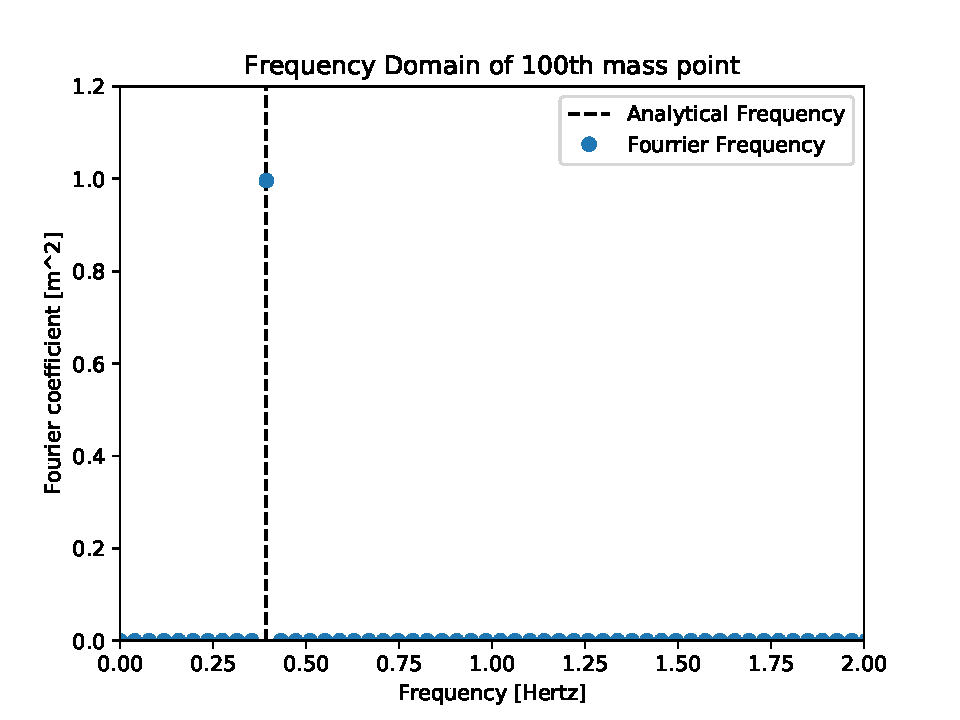
\includegraphics[width=\textwidth]{../fig/100_point_fourier.pdf}
\caption{Frekvensspekteret til $y_{99}$ over frekvensintervallet $f\in [0\mathrm{Hz},\ 2\mathrm{Hz}]$}
\label{fig:100_point_fourier}
\end{figure}

Vi vet at et frekvensspekter av en sinusbølge med entydig frekvens kan vise flere frekvenser enn antatt dersom bølgen ikke er et heltall antar bølgelengder. Fordi vi driver med numeriske beregninger med begrenset oppløsning forventer vi at vi ikke har klart å få et nøyaktig heltall antall bølgelengder. Dette kan vi se effekten av i figur \ref{fig:100_point_fourier2}, der vi ser at vi så vidt har fått med oss noen frekvenser i nærheten av vår faktiske frekvens. Disse er riktignok ekstremt små, som tyder på at vår modell er meget god.
\begin{figure}[H]
\centering
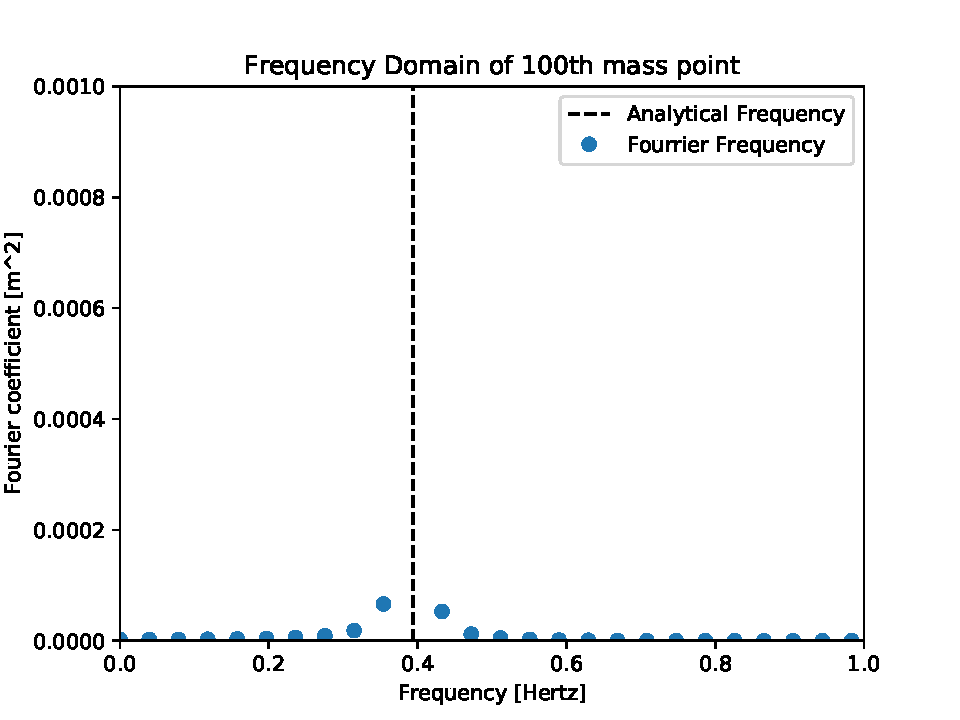
\includegraphics[width=\textwidth]{../fig/100_point_fourier2.pdf}
\caption{Forstørret frekvensspekter til $y_{99}$ over frekvensintervallet $f\in [0\mathrm{Hz},\ 1\mathrm{Hz}]$}
\label{fig:100_point_fourier2}
\end{figure}




\section*{Oppgave 6}
\subsubsection*{Teori og implementasjon}
Den totale energien til systemet vil bestå av kinetisk og potensiell energi. Vi diskretiserer begge energiene over de $N$ massepunktene.

Den kinesiske energien kommer fra hastigheten til hvert massepunkt $m_i$, som til sammen blir:
\begin{align*}
E_{k,total} = \sum\limits_{i=0}^{N} E_{ki} = \sum\limits_{i=0}^{N}\frac{1}{2}m_i v_i^2
\end{align*}
Hastigheten til hvert punkt er riktignok ikke noe vi har liggende eksplisitt, og vi må finne en måte å regne ut denne. For størst mulig nøyaktighet bruker vi den symmetriske topunktsformelen for derivasjon til å tilnærme hastigheten fra posisjonen til punktet på to tidspunkter. Hastigheten til punktet $y_i^0$ blir da
\begin{align*}
v_i^0 \approx \frac{y_i^+ - y_i^-}{2\Delta t}
\end{align*}

Fra Hooke's har vi at den potensielle energien til en fjær med fjærkonstant $k$ som er utstrakt en lengde $\Delta y$ fra sitt likevektspunkt er gitt som $E_p = k\Delta y^2$. Summen av den potensielle energien til hver av de $N-1$ fjærene (kan også sees på som par av to og to massepunkt) blir da
\begin{align*}
E_{p,total} = \sum\limits_{i=0}^{N-1} E_{pi} = \sum\limits_{i=0}^{N-1} 0.5k(\Delta y_i)^2 = \sum\limits_{i=0}^{N-1} 0.5k(y_{i+1} - y_i)^2
\end{align*}

Dersom vår numeriske implementasjon er tilstrekkelig nøyaktig skal summen av disse være konstant.

\subsubsection*{Resultat}
Figur \ref{fig:energy_cons} viser den kinetiske og potensielle energien over tid, samt summen av dem. Jeg har valgt å bare plotte energien i de første fem periodene, for at det skal bli tydeligere. Som vi ser virker den totale energien å være meget godt bevart. Vi ser også at den kinetiske og potensielle oscillerer om hverandre i 5 perioder, som stemmer overens med systemet vi ser på. Når den stående bølgen er på sitt maksimale utslag, står den stille og har ingen kinetiske energi, men mye potensiell energi. Når utslaget er null over hele bølgen, har den ingen potensiell, men mye kinetisk energi. Vi ser også at både potensiell og kinetisk energi når 0 ved hver oscillasjon, som forventet. 
\begin{figure}[H]
\centering
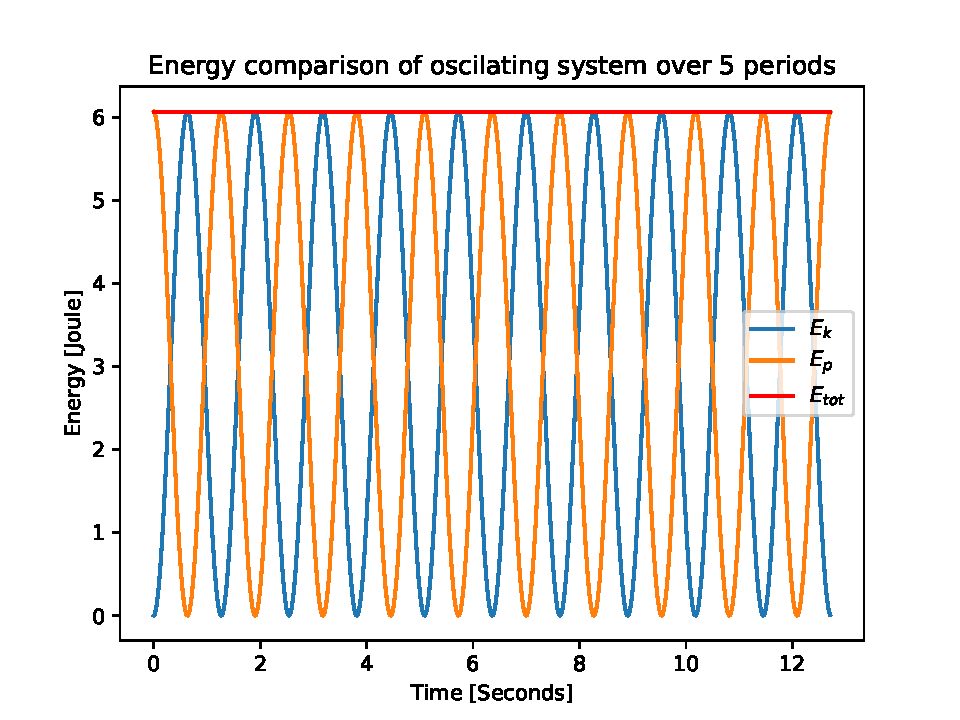
\includegraphics[width=\textwidth]{../fig/energy_cons.pdf}
\caption{Kinetisk, potensiell og total mekanisk energi til systemet over 5 svingeperioder med $\Delta t = \SI{0.01}{s}$}
\label{fig:energy_cons}
\end{figure}


Figur \ref{fig:energy_cons2} viser et meget forstørret bilde av bare den totale energien til systemet. Den rød linjen viser systemet vi har sett på hittil, med $\Delta t = \SI{0.01}{s}$, men jeg har også inkludert lavere tidssteg for å demonstrere at oscillasjonen i den totale energien avtar etterhvert som presisjonen øker. Dette er et meget godt tegn på at vår implementasjon av systemet er som det skal. Vi ser tydelig at den totale energien kollapser til en konstant ved høyere presisjon.
\begin{figure}[H]
\centering
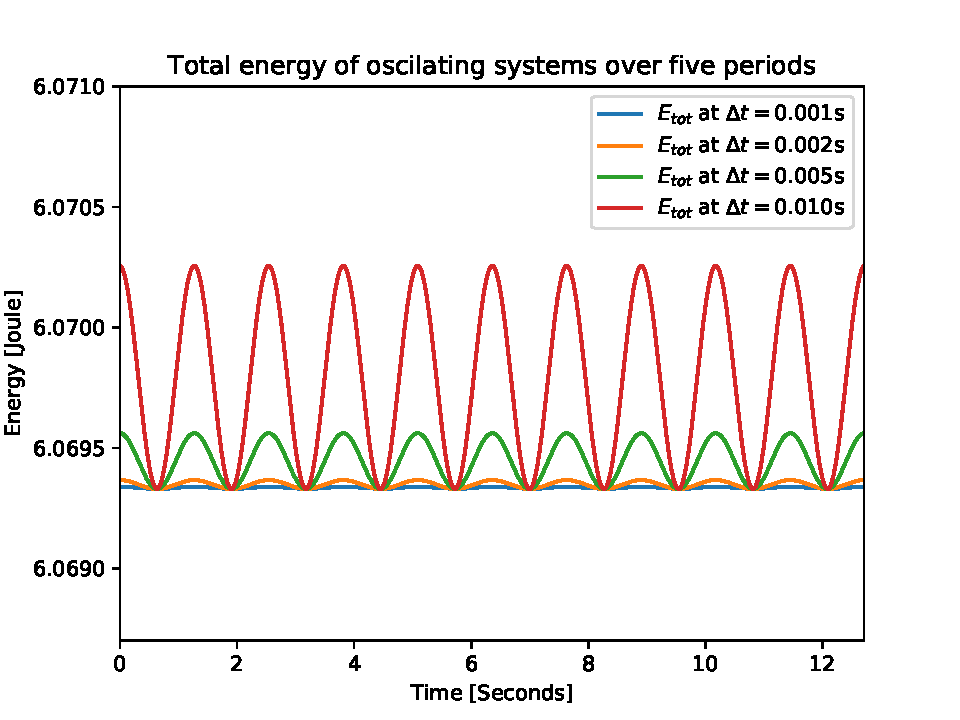
\includegraphics[width=\textwidth]{../fig/energy_cons2.pdf}
\caption{Total energi til fire systemer med varierende tidssteg over 5 perioder.}
\label{fig:energy_cons2}
\end{figure}

Figur \ref{fig:energy_cons3} viser energibevaringen til systemet vårt over 1000 perioder. Dette er for å demonstrere at systemet ikke blir utstabilt over tid. Vi ser at den totale energien virker meget stabil, selv over lang tid.
\begin{figure}[H]
\centering
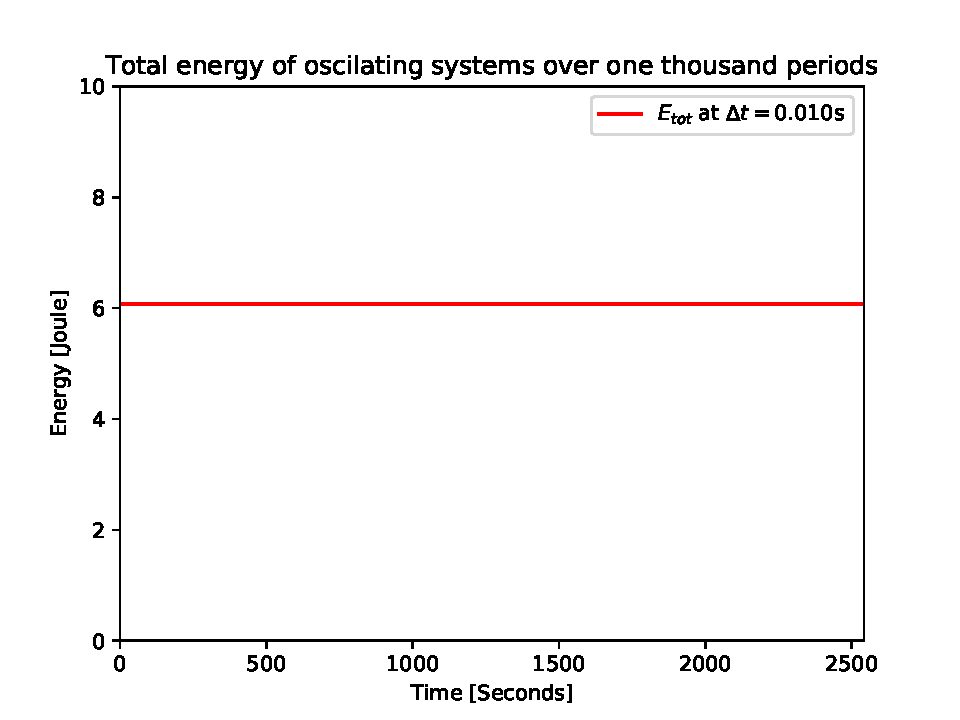
\includegraphics[width=\textwidth]{../fig/energy_cons3.pdf}
\caption{Kinetisk, potensiell og total mekanisk energi til systemet over tid.}
\label{fig:energy_cons3}
\end{figure}



\section*{Oppgave 7}
Å implementere denne initialbetingelsen er ganske simpelt. Vi bare setter hvert massepunkt til høyden spesifisert av den oppgitte funksjonen, både for $y^-$ og $y^0$. At disse to initialposisjonene er like betyr at vi ikke forventer én bølge som beveger seg bortover med en hastighet $v_B$. Dette er fordi hvis vi hadde én bølge som beveget seg i x-retning hadde vi forventet at den beveget seg fra tiden $t^-$ til $t^0$, og at $y^-$ var forskjellig fra $y^0$.

De første sekundene av trekantbølgen er vist i figur \ref{fig:tri}. Her ser vi nettopp at vi ikke fikk én bølge, men heller en sammensetning av to bølger, som tilfeldigvis krysset hverandre og interfererte i tidspunktet vi startet i. Men hvorfor fikk vi ikke stående bølger, slik som vi fikk i oppgave 4, da vi satte $y^0 = y^-$? En stående bølge er nemlig ikke noe annet enn to bølger som beveger seg i motsatt retning, men for å få effekten vi så i oppgave 4 trenger vi at de er kontinuerlige planbølger, og ikke to enkelte bølgepakker, slik vi ser i denne oppgaven. Dersom vi modellerte flere trekantbølger i en kontinuerlig planbølge bortover, ville vi fått stående bølger.
 
I figur \ref{fig:tri2} ser vi hvordan bølgen utvikler seg videre etter å ha kollapset inn i to bølger. Begge bølgene går mot hver sin kant, og får en total refleksjon i møtet med endepunktene, fordi disse har uendelig masse, og derfor uendelig impedans, som gir en refleksjonskoeffisient lik den negative av den innkommende bølgen. Bølgene beveger seg deretter mot hverandre, og møtes i midten, der de interfererer til en ny trekantbølge, identisk til den vi startet med, bare negativ. Deretter fortsetter de tilbake til hver sitt endepunkt, og repeterer hele prosessen.

\begin{figure}[H]
\centering
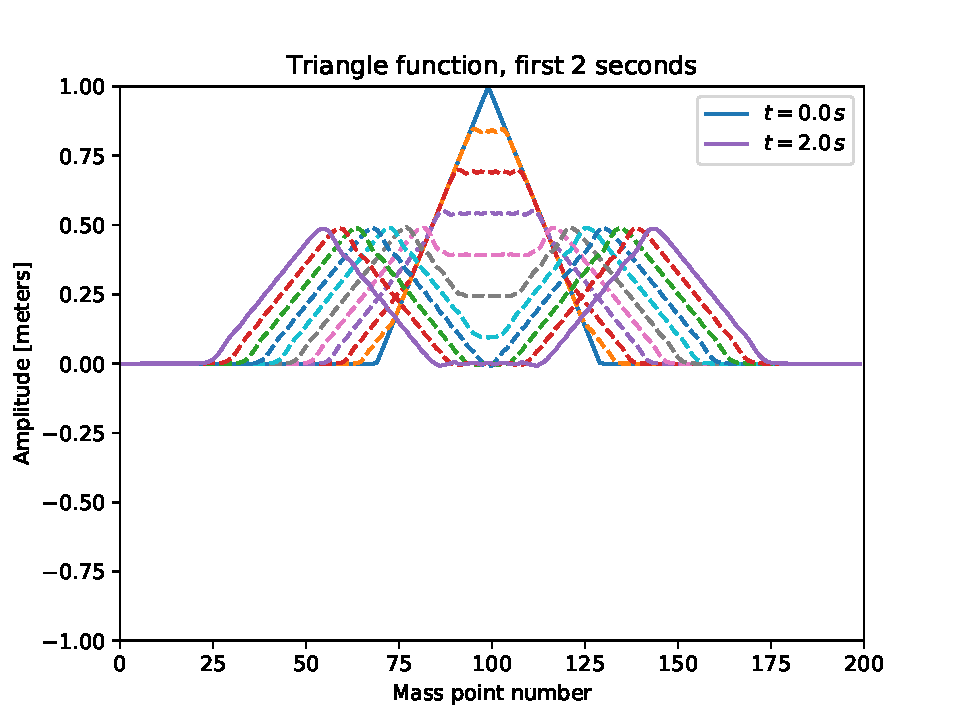
\includegraphics[width=\textwidth]{../fig/triangle_collapse.pdf}
\caption{Kollaps av trekantfunksjon til to andre funksjoner - første to sekunder.}
\label{fig:tri}
\end{figure}

\begin{figure}[H]
\centering
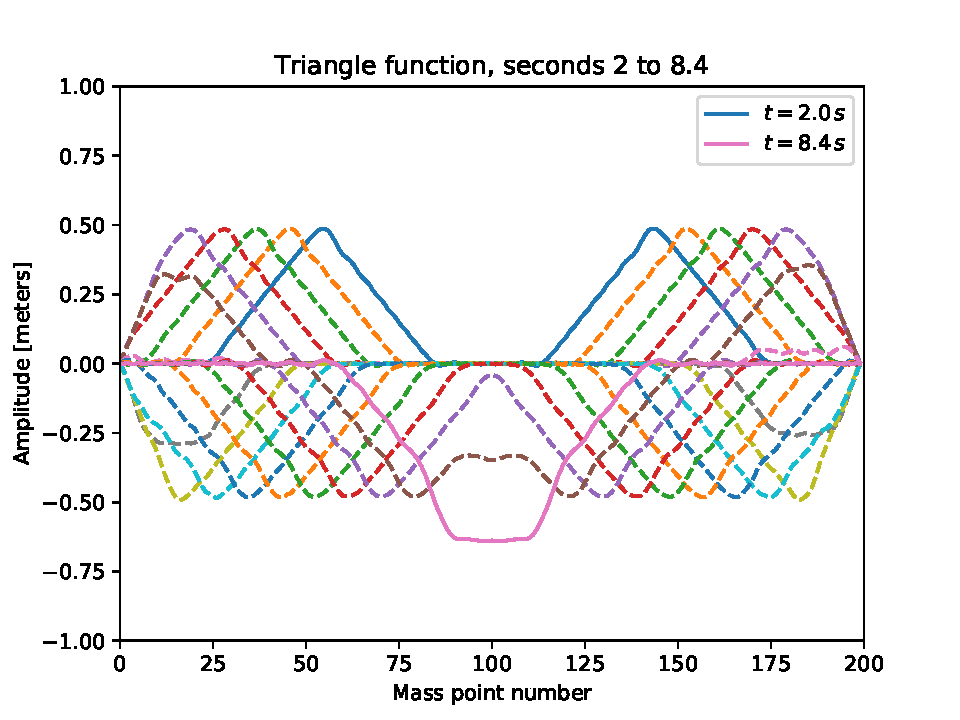
\includegraphics[width=\textwidth]{../fig/triangle_collapse2.pdf}
\caption{Utvikling av de to nye trekantfunksjonene over tid - 2 til 8.4 sekunder.}
\label{fig:tri2}
\end{figure}




\section*{Oppgave 8}
Vi kan først sentrere trekanten rundt punktet $i = 30$. I oppgave 7 studerte vi en trekant sentrert rundt punktet $i = 99$. Vi trenger altså bare å forskyve denne ligningen med 69 punkter:
\begin{equation}\label{eqn:initial}
y_i^0 = \begin{cases}
n/30 & \mathrm{if} 1 \leq i \leq 30 \\
(60-n)/30 & \mathrm{if}\: 31 \leq i \leq 59\\
0 & \mathrm{otherwise}
\end{cases}
\end{equation}

Da vi utledet bølgeligningen fant vi at bølgens utbredelseshastighet var gitt som
\begin{align*}
v_B = \sqrt{\frac{k}{m}}\Delta x
\end{align*}

I de forrige oppgavene har vi satt initialbetingelser som ikke oppfyller dette kriteriet, som betyr at bølgen må være en sammensetninger av flere bølger. Vi skal nå forsøke å oppfylle dette kriteriet, for å sitte igjen med én bølge som beveger seg til høyre.

Hvis bølgen beveger seg $n$ massepunkter i løpet av et tidssteg $\Delta t$, vil det bety at bølgen beveger seg med en hastighet
\begin{align*}
v_B = \frac{n\Delta x}{\Delta t}
\end{align*}

Setter vi dette lik vår analytiske bølgehastighet fra bølgeligningen, får vi en betingelser
\begin{align*}
\sqrt{\frac{k}{m}}\Delta x &= \frac{n\Delta x}{\Delta t}\\
\Delta t &= n\sqrt{\frac{m}{k}}\\
\end{align*}
For at vi bare skal ha en bølge har vi altså en betingelse på relasjonen mellom $\Delta t$, og antallet punkter bølgen beveger seg i løpet av dette tidssteget, $n$. Dette kan vi bruke til å sette en initialbetingelse som gir bølgen vi ønsker, ved å velge hvor langt tilbake vi ønsker å sette $y^-$, og velge en korrekt $\Delta t$ til dette.

Det vil være enklere å sette $y^-$ på samme form som ligning \ref{eqn:initial}, altså en trekant med et veldefinert toppunkt. Dette vil innebære å sette $n$ til et heltall, og flytte trekanten et heltall antall punkter tilbake. Det vil selvsagt være mulig å sette $n$ til noe annet enn et heltall, men dette vil innebære at vi må interpolere bølgens posisjon for å finne initialbetingelsene. Vi ser at dersom vi ønsker at $n$ skal være et heltall har vi bare ett alternativ, som er $n=1$. Vi husker fra ligning \ref{eqn:dt} at vi har en betingelse på $\Delta t$ som krever at
\[\Delta t \leq \sqrt{\frac{m}{k}} \]

Vi definerer altså nå $\Delta t = \sqrt{\frac{m}{k}}$, og setter $y^-$ ett massepunkt til venstre for $y^0$. Dette tilsvarer betingelsen
\begin{align*}
y_i^- = y_{i-1}^0
\end{align*}
Som resulterer i en trekant sentrert rundt punktet $i = 29$.

Figur \ref{fig:tri3} viser trekantens bevegelse. Vi ser den beveger seg som forventet mot høyre, for den treffer den uendelige impedansovergangen ved høyre vegg, og snur til å bli negativ. Oppførselen er i utgangspunktet likt med hver av de to bølgene vi så i oppgave 7.

\begin{figure}[H]
\centering
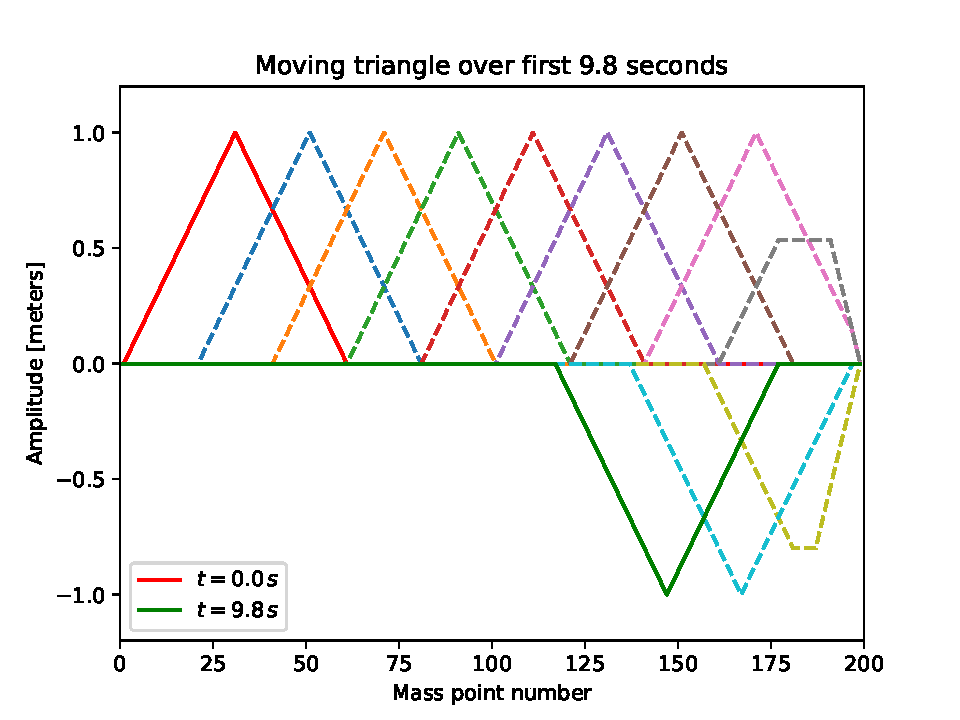
\includegraphics[width=\textwidth]{../fig/moving_triangle.pdf}
\caption{Bevegelse av trekantfunksjonen de første 9.8 sekundene.}
\label{fig:tri3}
\end{figure}


\section*{Oppgave 9}
Vi vet at transmisjon og refleksjonskoeffisientene til en bølge som går gjennom en impedansovergang er gitt som
\begin{align}\label{eqn:T}
T &= \frac{A_t}{A_i} = \frac{2Z_0}{Z_1+Z_0}
\end{align}
\begin{align}\label{eqn:R}
R &= \frac{A_r}{A_i} = \frac{Z_0-Z_1}{Z_0+Z_1}
\end{align}
Der $Z_0$ er impedansen før overgangen og $Z_1$ er impedansen etter.


Vi løser ligning \ref{eqn:T} med hensyn på impedansforholdet $Z_1/Z_0$:
\begin{align*}
T = \frac{2Z_0}{Z_1+Z_0} \quad \implies \quad TZ_1 + TZ_0 = 2Z_0 \\
TZ_1 = Z_0(2-T) \quad \implies \quad \frac{Z_1}{Z_0} = \frac{2-t}{T}
\end{align*}

Vi gjør tilsvarende for ligning \ref{eqn:R}.
\begin{align*}
R = \frac{Z_0-Z_1}{Z_0+Z_1} \quad \implies \quad RZ_0 + RZ_1 = Z_0 - Z_1 \\
Z_1(R+1) = Z_0(1-R) \quad \implies \quad \frac{Z_1}{Z_0} = \frac{1-R}{R+1}
\end{align*}

Vi kan finne amplituden til den transmitterte og reflekterte bølgen ved å se etter maksimalt positivt og negativt utslag til bølgen etter den har gått over impedansovergangen. Printer vi ut dette fra programmet får vi at
\begin{lstlisting}[frame=single]
Amplitude of transmitted wave = 0.711 m
Amplitude of reflected wave = -0.277 m
\end{lstlisting}
Ettersom amplituden til den innkommende bølgen er 1, vil vi få at $T = A_t/A_i = A_t$, og $R = A_r/A_i = A_r$.
Setter vi inn amplitudene inn i ligningene våre for impedans, får vi
\begin{align*}
\frac{Z_1}{Z_0} = \frac{2-T}{T} = \frac{2-A_t}{A_t} = \frac{2-\SI{0.711}{m}}{\SI{0.711}{m}} = 1.813
\end{align*}
Og
\begin{align*}
\frac{Z_1}{Z_0} = \frac{R+1}{1-R} = \frac{T_r+1}{1-T_r} = \frac{-0.277+1}{1+0.277} = 1.766
\end{align*}

Vi ser at den beregnede impedansen blir $Z = 1.813$, og $Z=1.766$ avhengig av hvilken av bølgene vi ser på.Forskjellen stammer sannsynligvis fra mangel på numerisk presisjon.

Vi kan sammenligne impedansen vi har regnet ut til den analytiske impedansen. Impendans til et medium er gitt som
\begin{align*}
Z = \sqrt{km}
\end{align*}
Vi får da at impedansovergangen blir
\begin{align*}
\frac{Z_1}{Z_0} = \frac{\sqrt{km_1}}{\sqrt{km_0}} = \frac{\sqrt{k3m_0}}{\sqrt{km_0}} = \sqrt{3} = 1.732
\end{align*}

Vi kan regne ut den analytiske amplituden som bølgene i teorien skal ha ved impedansovergangen, og se om den stemmer med vårt resultat. Figur \ref{fig:imp1} viser bølgens oppførsel idet den treffer impedansovergangen. Det er lagt inn horisontale linjer ved den analytiske amplituden til den transmitterte og reflekterte bølgen. Som vi ser treffer den reflekterte bølgen sin analytiske amplitude ganske godt, mens den transmiterte bølgen ligger litt under. Dette stemmer overens med at den utregnede impedansen fra den reflekterte bølgen var nærmere den analytiske løsningen enn den beregnede impedansen fra den transmitterte bølgen. Grunnen til at ingen av dem har spesielt stor nøyaktighet er at det oppstår en rekke mindre bølger i impedansovergangen, grunnet vår begrensede presisjon. Vi kan så vidt se disse små bølgene i figur \ref{fig:imp2}, som viser bølgens utvikling etter impedansovergangen.

\begin{figure}[H]
\centering
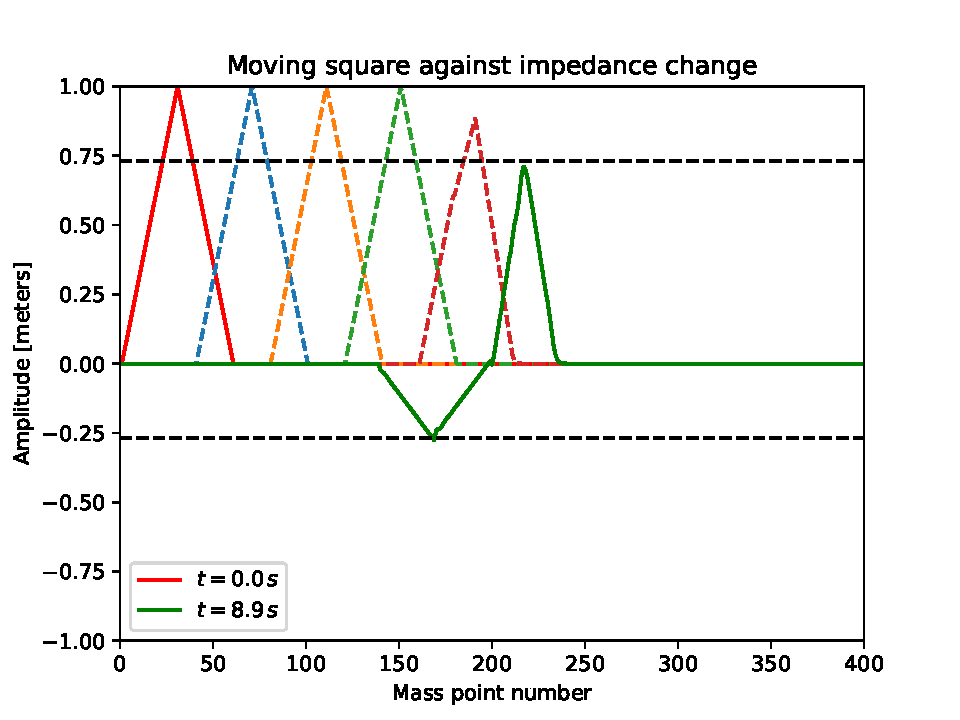
\includegraphics[width=\textwidth]{../fig/impedance.pdf}
\caption{Trekantbølge mot impedansovergang.}
\label{fig:imp1}
\end{figure}

\begin{figure}[H]
\centering
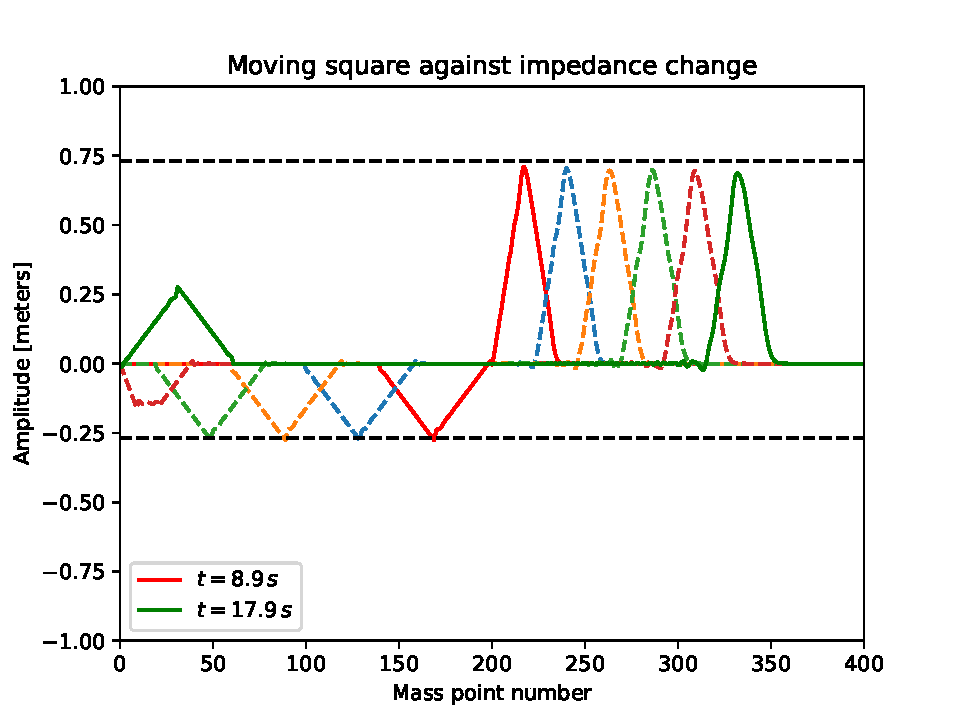
\includegraphics[width=\textwidth]{../fig/impedance2.pdf}
\caption{Trekantbølge etter impedansovergang.}
\label{fig:imp2}
\end{figure}




















\pagebreak
\section*{Appekdiks A - Utledning av to-punkts sentral differanse metoden}
Måle med denne utledningen er å tilnærme den dobbelt tidsderiverte av en funksjon ved hjelp av Taylor-ekspansjon. Vi skal tilnærme $\ddot{y_i}(x,t)$ ved å Taylorekspandere forover og bakover i tid, rundt $y(x,t)$.
\begin{align*}
y(x,t+\Delta t) = y(x,t) + \dot{y}(x,t)\Delta t + \frac{1}{2}\ddot{y}(x,t)\Delta t^2 + \frac{1}{6}\dddot{y}(x,t) \Delta t^3 + \mathcal{O}(\Delta t^4)\\
y(x,t-\Delta t) = y(x,t) - \dot{y}(x,t)\Delta t + \frac{1}{2}\ddot{y}(x,t)\Delta t^2 - \frac{1}{6}\dddot{y}(x,t) \Delta t^3 + \mathcal{O}(\Delta t^4)
\end{align*}
Legger vi sammen hver side av ligningene, får vi:
\begin{align*}
y(x, t+\Delta t) + y(x, t-\Delta t) = 2y(x,t) + 2\frac{1}{2}\ddot{y}(x,t)\Delta t^2 + \mathcal{O}(\Delta t^4)
\end{align*}
Som vi kan løse for $\ddot{y}$:
\begin{align*}
\ddot{y}(x,t) = \frac{y(x, t+\Delta t) -2y(x,t) + y(x, t-\Delta t)}{\Delta t^2} + \mathcal{O}(\Delta t^4)
\end{align*}
På deskritisert form blir dette
\begin{align}
\ddot{y}_i^0 \approx \frac{y_i^+ - 2y_i^0 + y_i^-}{\Delta t^2}
\end{align}
Der vi har har en presisjonsfeil som går som $\Delta t^4$. 


\pagebreak
\section*{Appendiks B - Python kode}
Koden kan også finnes på følgende github adresse:

\url{https://github.com/asdfbat/FYS2130/tree/master/Prosjektoppgave/src}

Kopiering av kode fra PDF gir ofte litt problemer med indentering, og innimellom også non-ASCII tegn.

\subsection*{Oppgave 4)}
\inputminted[frame=single, fontsize=\footnotesize]{python}{../src/oppgave4.py}

\pagebreak
\subsection*{Oppgave 5)}
\inputminted[frame=single, fontsize=\footnotesize]{python}{../src/oppgave5.py}

\pagebreak
\subsection*{Oppgave 6)}
\inputminted[frame=single, fontsize=\footnotesize]{python}{../src/oppgave5.py}

\pagebreak
\subsection*{Oppgave 7)}
\inputminted[frame=single, fontsize=\footnotesize]{python}{../src/oppgave5.py}

\pagebreak
\subsection*{Oppgave 8)}
\inputminted[frame=single, fontsize=\footnotesize]{python}{../src/oppgave5.py}

\pagebreak
\subsection*{Oppgave 9)}
\inputminted[frame=single, fontsize=\footnotesize]{python}{../src/oppgave5.py}


\end{document}



